\chapter{From Primitive Survival to Digital Domination}

\section{The Competitive Nature of Humanity}

Humanity’s relentless pursuit of \textbf{superiority, recognition, and dominance} has been a constant throughout history. From early survival strategies to the era of modern technology, the drive to \textbf{outperform others} has been a decisive factor in advances across science, warfare, politics—and, more recently, digital realms.

This competitive impulse goes beyond simple ambition; it is a \textbf{deeply ingrained psychological mechanism} that has shaped human behavior for centuries. As \textcite{festinger1954theory} explained through his \textbf{Social Comparison Theory}, individuals are naturally inclined to evaluate themselves against their peers, a process that reinforces competition by seeking validation and status. In a similar vein, \textcite{mcclelland1961achievement} introduced the \textbf{Achievement Motivation Theory} to demonstrate that the inherent desire to succeed and surpass others is crucial not only for personal fulfillment but also for social standing.

Viewed from an \textbf{evolutionary perspective}, competition has been essential for survival. Early human societies relied on traits such as strategic thinking, adaptability, and cooperative behaviors to secure resources, defend territories, and outcompete rival groups. Over time, these traits not only ensured survival but also influenced the development of complex \textbf{cultural, intellectual, and economic systems}. Even from a young age, individuals instinctively compare themselves with others, perpetuating a competitive framework embedded in our cognition and social interactions.

\begin{quote}
\textbf{\textit{What began as a survival mechanism has evolved into a multifaceted force that continues to shape human ambition and societal progress.}}
\end{quote}

The advent of modern technology has transferred this age-old drive into \textbf{digital environments}. The development of \textbf{computers} and the emergence of the \textbf{internet} revolutionized human interaction, information processing, and competitive engagement. In particular, video games have emerged as a potent platform that encapsulates competitive spirit through structured, goal-oriented systems—offering challenges against both artificial intelligence and human opponents.

These digital platforms mirror the essence of traditional competition by demanding skill optimization, the discovery of hidden mechanics, and the exploitation of strategic advantages. Empirical studies reveal that under competitive pressure, individuals are prone to seek alternative methods to gain an edge, especially when conventional avenues for success are obstructed \parencite{murdock2001cheating}. In the realm of online multiplayer gaming, the presence of \textbf{ranking systems, leaderboards, and social validation} further intensifies this competitive drive, urging players to pursue victory through mastery, strategy, or—even through exploitation.

To grasp how competition has been reinvented in the digital age, it is necessary to explore the historical evolution that laid the groundwork for these advancements. The subsequent sections will trace the development of \textbf{computation}, the advent of \textbf{networked systems}, and the rise of \textbf{video games} as dominant cultural and competitive forces. Through this historical lens, we reveal how ancient competitive instincts have been transposed into virtual battlegrounds where \textbf{skill, innovation, and adaptability} are the keys to success.

\section{The Birth of Computation and the Internet: A New Digital Battleground}

The roots of digital competition lie in humanity’s enduring efforts to \textbf{automate reasoning and computation}. From rudimentary counting devices to complex mechanical systems, civilizations have continually sought to enhance their ability to solve mathematical problems—an essential skill for the advancement of commerce, astronomy, and engineering.

\subsection{Early Computational Tools: From the Abacus to Mechanical Calculators}

To improve accuracy and efficiency in arithmetic operations, ancient societies devised tools that supported numerical reasoning. Among the earliest was the \textbf{abacus} (circa 2400 BCE), which saw widespread use in Mesopotamia, China, and Europe. This manually operated device enabled rapid calculations and laid the groundwork for future developments in computational thinking.

By the 17th century, the integration of mechanical engineering into mathematical problem-solving gave rise to more sophisticated inventions. One notable example is \textbf{Pascal’s Adding Machine} (1642), designed by \textbf{Blaise Pascal}. This mechanical calculator employed interlocking gears to automate basic arithmetic, significantly reducing the cognitive load of manual computation and heralding a shift toward mechanized processing.

\subsection{The 19th-Century Revolution: The Birth of Programmable Machines}

While earlier devices focused on performing fixed calculations, the 19th century introduced a paradigm shift with the conceptualization of \textbf{programmable machines}. Central to this revolution was \textbf{Charles Babbage}, whose design for the \textbf{Analytical Engine} introduced the foundational principles of modern computing, including conditional branching, memory storage, and modular input/output.

Expanding on Babbage’s work, \textbf{Ada Lovelace} recognized that such machines could go beyond numerical tasks. Her algorithm for the Analytical Engine is widely regarded as the first computer program. More significantly, her insights into symbolic computation and algorithmic design anticipated the emergence of \textbf{general-purpose computing} and modern programming languages.

\subsection{The Acceleration of Computation in the 20th Century}

The 20th century brought exponential advances in computing, driven largely by scientific innovation and geopolitical demands. The transition from mechanical apparatuses to fully electronic systems revolutionized data processing, transforming computation into a critical enabler of technological and industrial growth.

\subsubsection{World War II and the Role of Computation}

The exigencies of \textbf{World War II} played a pivotal role in accelerating computational innovation. \textbf{Alan Turing}'s formulation of the \textbf{Turing Machine} provided the theoretical framework for algorithmic processing, while his practical work in cryptanalysis at Bletchley Park—particularly in deciphering the \textbf{Enigma cipher}—demonstrated the immense strategic value of computational power.

Simultaneously, pioneering machines such as \textbf{Colossus} (UK, 1943) and \textbf{ENIAC} (US, 1945) were developed to perform large-scale calculations for military applications, including cryptography and ballistic modeling. These efforts illustrated how computation could surpass human limitations, laying the foundation for a new era of machine-assisted problem solving.

\subsubsection{Post-War Expansion: From Military to Commercial Computing}

In the aftermath of the war, computing technologies rapidly extended into academic research, industrial automation, and eventually the consumer market. The invention of the \textbf{transistor} in 1947, followed by the development of \textbf{integrated circuits}, enabled a dramatic reduction in size, cost, and power consumption of computing devices.

By the 1970s and 1980s, companies such as \textbf{IBM}, \textbf{Apple}, and \textbf{Microsoft} were instrumental in the democratization of computing. Their contributions led to the widespread adoption of \textbf{personal computers}, transforming what was once an industrial tool into an everyday instrument for work, education, and entertainment.

\subsection{The Birth of the Internet: From Military Networks to Global Infrastructure}

Despite the growing capabilities of standalone computers, a true revolution emerged with the advent of \textbf{networked computing}. Initiated in the late 1960s, the \textbf{ARPANET} project—funded by the U.S. Department of Defense—introduced the concepts of \textbf{decentralized communication} and \textbf{packet switching}, allowing data to be transmitted in more reliable and efficient ways.

The subsequent standardization of \textbf{TCP/IP protocols} in the early 1980s enabled the seamless interconnection of disparate networks, laying the groundwork for the modern \textbf{Internet}. The introduction of the \textbf{Domain Name System (DNS)} in 1984 further simplified access to networked resources by replacing numeric IP addresses with human-readable names.

A transformative milestone occurred in 1991, when \textbf{Tim Berners-Lee} developed the \textbf{World Wide Web}, a hyperlinked system that provided a user-friendly interface for navigating online information. This innovation catalyzed a massive expansion in digital communication, turning the internet into a \textbf{global infrastructure} by the mid-1990s—enabling not only communication and commerce, but also the emergence of \textbf{competitive digital ecosystems} where individuals and organizations could engage, create, and compete on an unprecedented scale.
\subsection{The Digital Arena: From Computing to Competition}

As computational capabilities expanded and network infrastructures matured, new forms of competition began to emerge within digital spaces. Informal gaming gatherings—held in LAN parties and cybercafés—provided the cultural groundwork for organized digital play. These early communities, driven by curiosity and technical experimentation, laid the foundation for a broader transformation in how games were perceived and played.

\begin{figure}[h!]
    \centering
    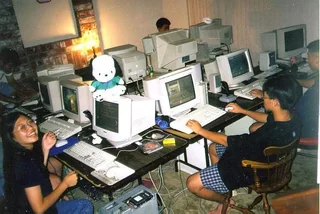
\includegraphics[width=1\linewidth]{images/quakelan.png}
    \caption{LAN party in the late 1990s—a grassroots precursor to modern esports.}
    \label{fig:lanparty}
\end{figure}

The rise of online gaming redefined digital entertainment as a structured and competitive experience. The introduction of \textbf{matchmaking systems}, \textbf{ranking ladders}, and \textbf{persistent progression mechanics} transformed casual play into continuous skill-based challenges. Pioneering titles such as \textbf{Quake}, \textbf{Counter-Strike}, and \textbf{StarCraft} set the standard for modern competitive games, combining reflex-based gameplay with strategic depth.

These systems offered players clear feedback loops—performance metrics, leaderboards, win/loss ratios—that fueled their desire to improve and dominate. As a result, gaming began to evolve from a leisure activity into a compelling arena of personal achievement and social recognition.

\subsection{From Networks to Virtual Battlefields}

The transformation of video games into \textbf{virtual battlefields} was fueled by technological advancements, global connectivity, and the rise of online communities. With real-time multiplayer becoming the norm, players worldwide could compete instantly, honing tactics and strategies to achieve recognition.

Video games offered an ideal competitive environment: \textbf{clear rules}, \textbf{quantifiable performance}, and \textbf{equal access}. As participation expanded, so did the supporting infrastructure—grassroots tournaments evolved into professional leagues, and casual players into sponsored competitors.

This convergence of entertainment, technology, and sport gave rise to \textbf{esports}, a global industry with professional teams, media coverage, and multimillion-dollar prize pools. What began as leisure became a legitimate career path and a powerful cultural force.

The same instinct that once ensured survival now drives mastery in digital arenas, where \textbf{technical skill, cognitive agility}, and \textbf{strategic thinking} define success.

The next chapters examine how this competitive landscape has also fostered new forms of rule-breaking. We will explore the evolution of \textbf{cheating} as both a technical challenge and a cultural phenomenon, revealing how players manipulate systems designed to ensure fair play.
